\chapter{Udvikling}\label{kapitel_Udvikling}

I dette afsnit findes et udsnit af kravspecifikationen, herunder en beskrivelse af de aktuelle aktører, en beskrivelse af UC-funktionaliteter samt en fully dressed UC af UC2.

\section{Kravspecifikation}


\subsection{Aktørbeskrivelse}
\begin{longtabu} to \linewidth{@{}l l X[j]@{}}
    \textbf{Aktørnavn} &        \textbf{Type} &    \textbf{Beskrivelse}\\[-1ex]
    \midrule
    Sundhedsfagligt personale &    Primær &    Aktøren starter, foretager og afslutter målingen. Aktøren skal have relevans i henhold til en operationsstue samt have kendskab til proceduerne herved\\
        Tekniker &       Primær &    Kalibrerer systemet\\
    Transducer &        Sekundær &    Transduceren omsætter tryk til et analogt elektrisk signal\\
    Database &        Sekundær &    Måledataene gemmes i databasen.\\

    
\caption{Aktørbeskrivelse}\\
\label{actortable}
\end{longtabu}

\subsection{Use case diagram}
UC-diagrammet viser funktionaliteten af systemet.
\begin{figure}[H]
\centering
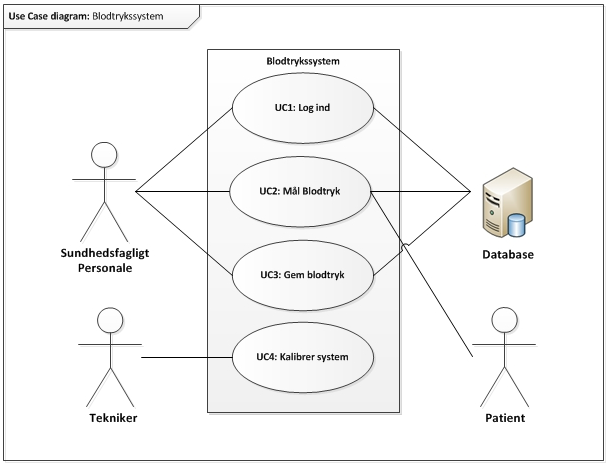
\includegraphics[scale=0.95]{uc.PNG}
\caption{Use case diagram}
\end{figure}

\subsection{Use case beskrivelser}


\subsubsection{Use case 1: Log ind}
For at kunne bruge systemet til blodtryksmåling, skal sundhedsfagligt personale logges ind. Dette gøres ved at indtaste korrekt ID med tilhørende kode, hvorefter der trykkes på "\textit{Log ind}"\- -knappen. Log ind-vinduet lukkes ned, og Diagnostik-vinduet vises. 


\subsubsection{Use case 2: Hent patientdata}
Før nulpunktsjusteringen kan foretages, skal patientens oplysninger angives. Dette gøres ved, at sundhedsfagligt personale indtaster patientens CPR-nummer og trykker på knappen "\textit{Hent patientoplysninger}"\- -knappen. Herefter angives patientens navn og CPR-nummer i Diagnostisk-vinduet. 

\subsubsection{Use case 3: Nulpunktsjustering}
Inden blodtryksmålingen kan foretages, skal systemet nulpunktsjusteres. Systemet foretager nulpunktsjustering efter at sundhedsfagligt personale har trykket på "\textit{Nulpunktsjustering}"\- -knappen. Herefter vises blodtrykket i Diagnostik-vinduet.

\subsubsection{Use case 4: Alarmer}
Systemet alarmerer sundhedsfagligt personale når blodtrykket bliver for højt eller lavt. Alarmeringen angives med lyd, hvorpå sundhedsfagligt personale har mulighed for at sætte systemets alarm på lydløs 

\subsubsection{Use case 5: Filtrer signal}
Sundhedsfagligt personale skal have mulighed for at slå det digitale filter til og fra. Dette gøres ved hjælp af "\textit{Til/fra}"\- -knappen.

\subsubsection{Use case 6: Gem data}
Systemet skal kunne gemme målingsdata. For at gemme data, trykker sundhedsfagligt personale på "\textit{Gem data}"\- -knappen, hvorefter måledata gemmes i databasen og systemet giver beskeden "\textit{Data gemt}"

\subsubsection{Use case 7: Kalibrer system}
Systemet kalibreres ved at tekniker påtrykker systemet tre kendte tryk. Herefter aflæser hen responserne på brugergrænsefladen og noterer afivgelserne fra de kendte tryk. Tekniker justerer så afvigelserne i systemets software, og systemet er kalibreret. 

\subsection{Fullydressed use case for use case X}
En direkte kopiering af tabellen fra Dokumentation, så ændringer fra ene dokument automatisk opdateres i andet.


\section{Systemarkitektur}
Også direkte kopieringer fra Dokumentation.

\subsection{Hardware}

\subsection{Software}


\section{Produktet}

Udarbejdelsen af produktet i hardware og software under iterationsprocessen med design, implementering og test.

\subsection{Hardware}

\subsection{Software}


\section{Accepttest}

For udvalgt use case.


\section{Opfyldelse af kravspecifikation}
Vurdering af accepttestens resultat.


\section{Videreudvikling}
Videreudvikling af selve produktet.
